\chapter{Memory}

Now, we move on to another major component in the computer: Memory. The discussion of memory will include Cache, Main Memory, and Secondary Memory (Disk). In this chapter, we will look at the Main Memory and Disk.

\section{Memory Hierarchy}
Previously, we talked about combinational circuits and sequential circuits. The first always gives the same output for a given set of inputs, while the latter stores information and provides output depending on the stored information. Therefore, we need to have materials to store information.

The maximum size of memory is determined by the addressing scheme. For example, a 16-bit address can only address \(2^{16} = 65,536\) memory locations. Most machines are byte-addressable, meaning each memory address location refers to a byte. Most machines retrieve or store data in words.

Also, there are some common abbreviations:
\begin{itemize}
  \item \(1\,\text{k} \approx 2^{10}\) (kilo)
  \item \(1\,\text{M} \approx 2^{20}\) (Mega)
  \item \(1\,\text{G} \approx 2^{30}\) (Giga)
  \item \(1\,\text{T} \approx 2^{40}\) (Tera)
\end{itemize}

Data transfer takes place through the \textbf{MAR} (Memory Address Register) and the \textbf{MDR} (Memory Data Register). Both MAR and MDR are located in the processor and are connected to memory via a bus. By using the address from the MAR, we can locate the required memory location, and then read from or write to it using the MDR.

\begin{minipage}{0.45\textwidth}
  The processor usually runs much faster than main memory. Small memories are fast, while large memories are slow. Leveraging this characteristic, we use \textbf{cache memory} to store data in the processor that is likely to be accessed soon. \\[5pt]
  Main memory is limited in size. To address this, we use \textbf{virtual memory} to increase the apparent size of physical memory by moving unused sections to disk. The translation between virtual and physical addresses is handled by the \textbf{Memory Management Unit (MMU)}. 
\end{minipage}
\begin{minipage}{0.5\textwidth}
  \begin{center}
  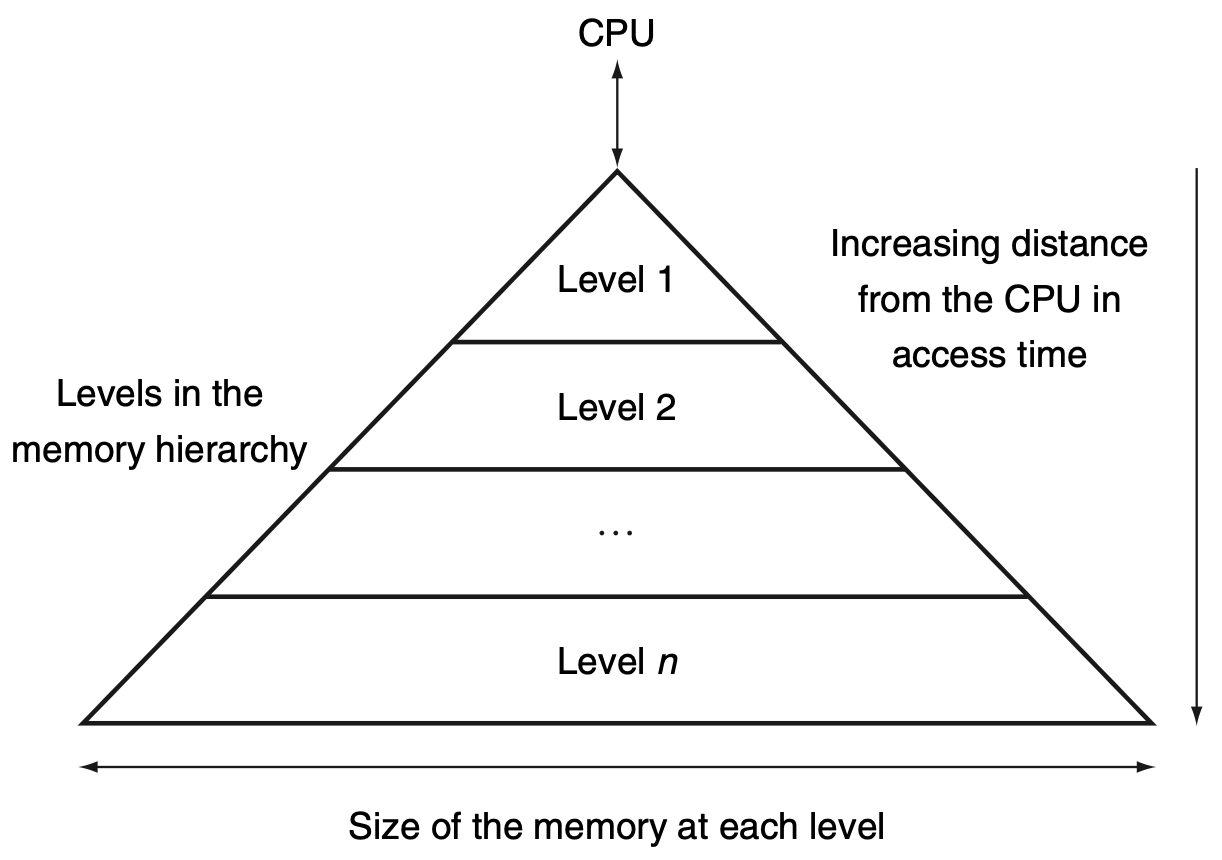
\includegraphics[width=\textwidth]{Figure/memory_struct.png}
\end{center}
\end{minipage}

We can visualize the memory hierarchy, which follows an \textbf{inclusive property}, meaning that data in Level 1 cache is a subset of that in Level 2, and so on up the hierarchy. 

We can view the memory hierarchy as follows: 
\begin{itemize}
  \item \textbf{Level 1 (L1)}: Cache using Static RAM (SRAM)
  \item \textbf{Level 2 (L2)}: Another level of cache, often using faster Dynamic RAM (DRAM)
  \item \textbf{Level 3 (L3)}: Main memory, typically DRAM
  \item \textbf{Level 4 (L4)}: Secondary memory such as flash storage or solid-state drives (SSD)
\end{itemize}

The first three levels consist of \textbf{volatile memory}, meaning they retain data only while power is on. In contrast, the secondary memory is \textbf{non-volatile} and retains data even when power is off.

As the distance from the CPU increases, so does the access time. Therefore, \textbf{Level 1 is the fastest}, and \textbf{Level 4 is the slowest}.

The above memory hierarchy works because of two types of locality. The first is \textbf{Temporal Locality} (locality in time), meaning that if a memory location is referenced, it will tend to be referenced again soon. It keeps the most recently accessed data items closer to the processor. The second is \textbf{Spatial Locality} (locality in space). If a memory location is referenced, the locations with nearby addresses will tend to be referenced soon. Therefore, we move blocks consisting of contiguous words closer to the processor.

For example, a variable array follows \textbf{Spatial Locality}, while a variable value follows \textbf{Temporal Locality}. 

Before moving into the next section, we now introduce some terminologies.

\begin{itemize}
  \item \textbf{Random Access Memory (RAM)} has comparable access time for any memory location.
  \item \textbf{Block (or line)} is the minimum unit of information that is present in a cache.
  \item \textbf{Hit Rate} is the fraction of memory accesses found in a level of the memory hierarchy.
  \item \textbf{Miss Rate} is the fraction of memory accesses not found in a level of the memory hierarchy.
  \item \textbf{Hit Time} is the time to access the block plus the time to determine hit or miss.
  \item \textbf{Miss Penalty} is the time to replace a block in that level with the corresponding block from a lower level.
  \item \textbf{Bandwidth} is the amount of data transferred per second when transferring a block of data steadily.
  \item \textbf{Latency} is the amount of time to transfer the first word of a block after issuing the access signal.
\end{itemize}

\begin{remark}
  Note that Hit Time is much smaller than Miss Penalty.
\end{remark}

\section{Information Storage}
We can store one bit of information using a pair of inverters, which is stable. However, if we want to change the value stored, we may replace the inverters with a NOR gate, resulting in the SR-Latch.

\begin{center}
  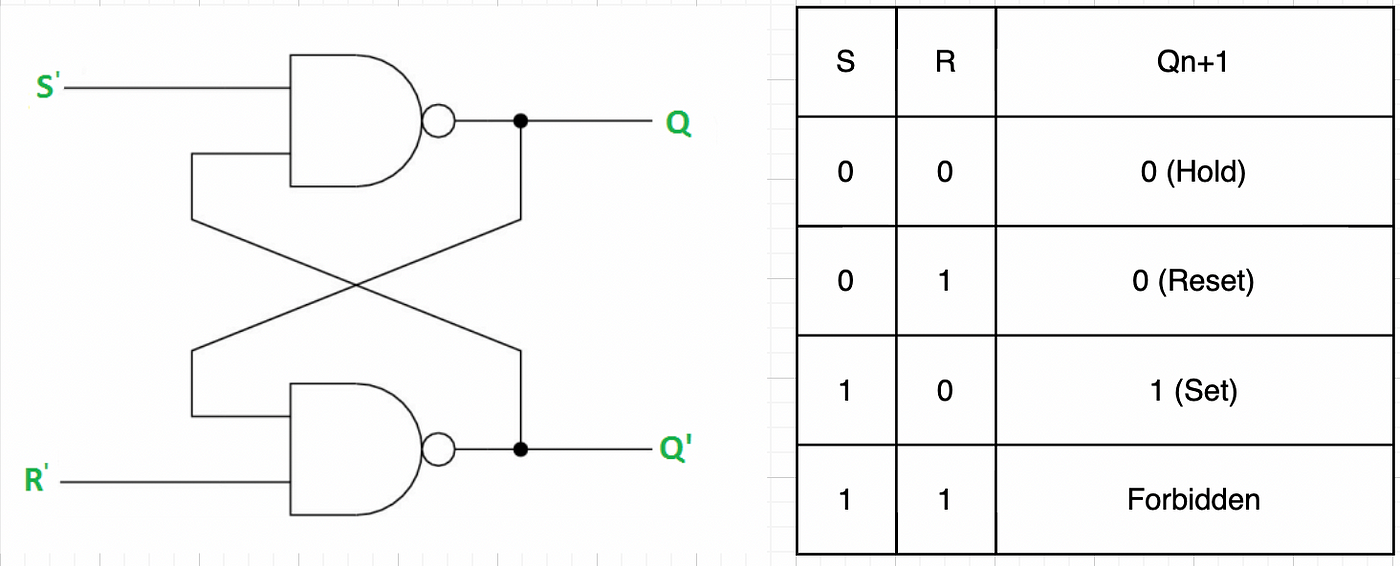
\includegraphics[width=0.6\textwidth]{Figure/SR_latch.png}
\end{center}

\begin{remark}
  S is set, R is reset. Thus, if \(S = 1\) and \(R = 0\), the latch is set, and the output will be 1.
\end{remark}

In SRAM cell, there are at least 6 transistors. This is used in most commercial chips, with a pair of weak cross-coupled inverters. Data is stored in the cross-coupled inverters, therefore, when power is applied, the data remains unchanged, making SRAM ``static''.

Since the data is stored in the cross-coupled inverters and doesn't need to be refreshed, it can be accessed quickly. However, SRAM cells require more transistors, which means they occupy more space on the chip.

In DRAM, there is only 1 transistor. It requires the presence of an external capacitor, and the modifications happen during the manufacturing process. For writing, we charge or discharge the capacitor. To read, charge redistribution takes place between the bit line and the storage capacitance.

The charge leaks away over time, so the data must be refreshed periodically to maintain it. This refresh cycle introduces additional latency compared to SRAM.

Because DRAM uses just a single transistor and a capacitor to store data, the DRAM cell is much smaller than an SRAM cell. This results in higher density, meaning more memory can be stored in the same physical space, making DRAM cheaper and suitable for larger memory sizes. So it’s commonly used for main memory in computers.

\section{Random Access Memory}
In the SRAM cell array, all rows are connected to a row decoder, and all columns are connected to a column selector and I/O circuits. Each intersection of the row and column represents a 6-T SRAM cell. One memory row holds a block of data, so the column address selects the requested bit or word from that block.

Here we call the row the \textbf{word line}, which refers to the horizontal lines. The vertical column lines are called \textbf{bit-lines}, which carry the data.

The arrangement in DRAM is similar, but each intersection represents a 1-T DRAM cell. The column address selects the requested bit from the row in each plane, with the row address determining which row is accessed first. The data in each cell is stored as a charge in a capacitor, and a transistor is used to access the charge.

The more common type used today is \textbf{Synchronous DRAM} (SDRAM), which uses a clock to synchronize its operations. This synchronization allows the refresh operation to become transparent to the user. Additionally, all control signals needed for operation are generated internally within the chip.

Normal SDRAM operates once per clock cycle, transferring data on either the rising or falling edge of the clock. In contrast, Double Data Rate (DDR) SDRAM transfers data on both the rising and falling edges of the clock, effectively doubling the data transfer rate compared to standard SDRAM.

\textbf{Static RAM (SRAM)} retains its state as long as power is applied. It is fast, consumes low power, but is costly to manufacture, which results in smaller capacity. SRAM is typically used for \textbf{Level 1 (L1)} and \textbf{Level 2 (L2)} caches inside processors.

\textbf{Dynamic RAM (DRAM)} stores data as an electrical charge on a capacitor. Because the charge leaks away over time, DRAM must be periodically refreshed to maintain the stored data. In exchange for this need for refreshing, DRAM offers much higher density compared to SRAM.

Going back to the previous memory hierarchy, the aim is to produce fast, large, and cost-effective memory. Therefore, \textbf{Level 1 (L1)} and \textbf{Level 2 (L2)} caches are usually implemented with \textbf{SRAM}, while the main memory is typically \textbf{DRAM}. This design leverages the principle of locality of reference to enhance performance.

In summary, \textbf{DRAM} is slow but cheap and dense, while \textbf{SRAM} is fast but expensive and not very dense.

\section{Interleaving}
A memory controller is normally used to interface between the memory and the processor. \textbf{DRAMs} have a slightly more complex interface as they require refreshing, and they usually have time-multiplexed signals to reduce the number of pins. \textbf{SRAM} interfaces are simpler and may not require a memory controller.

The memory controller accepts a complete address and the read or write signal from the processor. Then, the controller will generate the \textbf{Row Access Strobe} (RAS) and \textbf{Column Access Strobe} (CAS) signals. The high-order address bits, which select a row in the cell array, are provided first under the control of the \textbf{RAS} signal. Then, the low-order address bits, which select a column, are provided on the same address pins under the control of the \textbf{CAS} signal.

Based on the address given, data lines are connected directly between the processor and the memory.

SDRAM needs refreshing, but the refresh overhead is only less than 1 percent of the total time available to access the memory.

Again, as mentioned before, the processor and cache are fast, but the main memory is slow. Thus, we try to hide access latency by interleaving memory accesses across several memory modules. Each memory module has its own Address Buffer Register and Data Buffer Register, so they operate somewhat independently.

To perform memory module interleaving, two or more compatible memory modules are used. Within a memory module, several chips are used in ``parallel''.

For example, suppose we have a cache read miss and need to load from main memory. Assume a cache with an 8-word block, i.e., the cache line size is 8 words. Then, assume it takes one clock to send the address to DRAM memory and one clock to send the data back. In addition, DRAM has a 6-cycle latency for the first word, with each of the subsequent words in the same row taking only 4 cycles. Then for a single memory read, we have 
\[
  1 + 6 + 1 = 8 \text{ cycles}.
\]
\begin{center}
  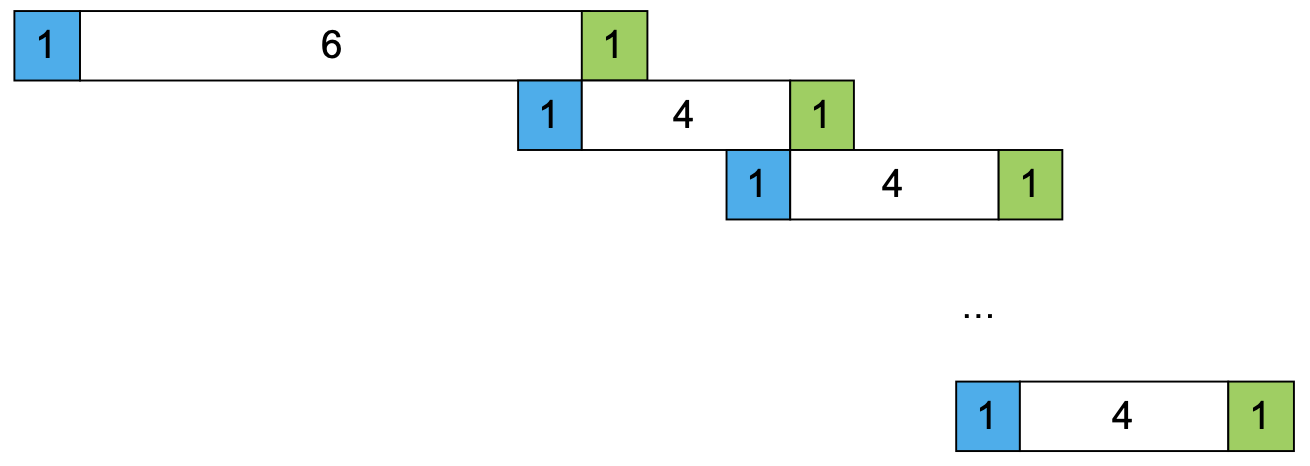
\includegraphics[width=0.6\textwidth]{Figure/overleaving_1.png}
\end{center}
And for the case of non-interleaving, there is no overlapping in cache access. Then all subsequent words in DRAM need 4 cycles. For example, if there are 8 reads, the total time required will be:
\[
  1 + 1 \times 6 + 7 \times 4 + 1 = 36 \text{ cycles}
\]
However, for four-module interleaving, we have 
\[
  1 + 6 + 1 \times 8 = 15 \text{ cycles}
\]
\begin{center}
  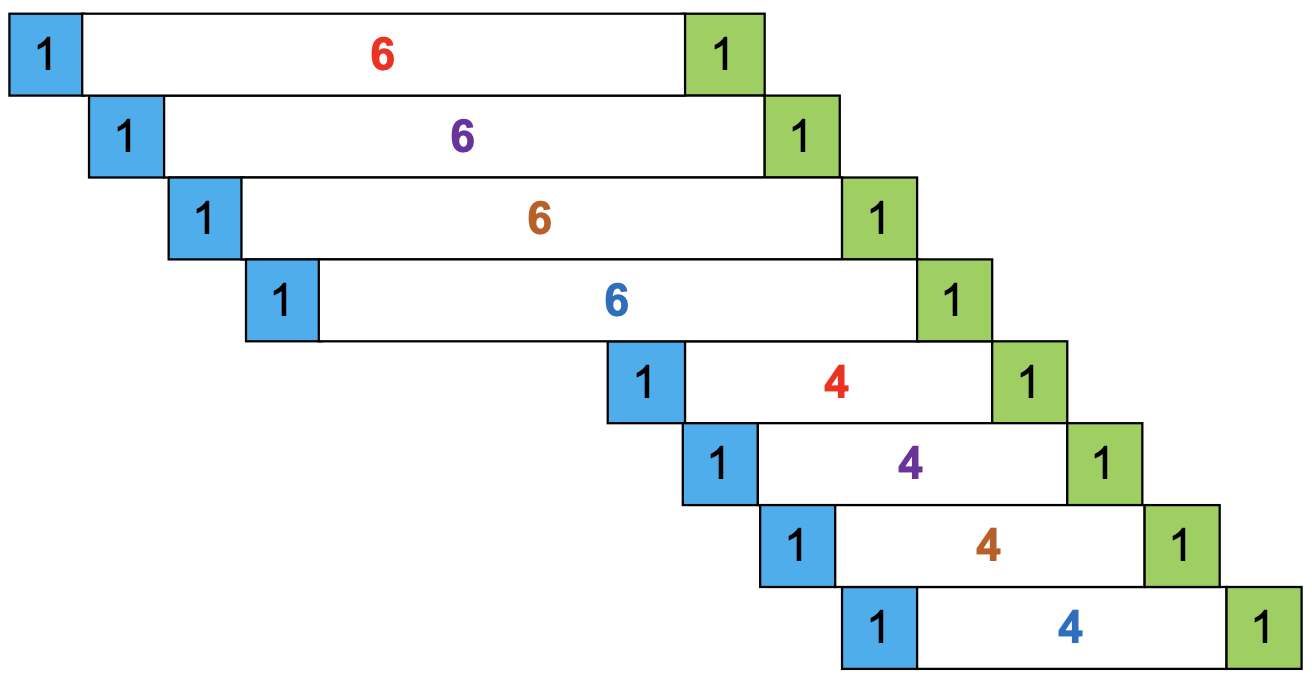
\includegraphics[width=0.6\textwidth]{Figure/overleaving_2.png}
\end{center}

\section{Secondary Memory}
Magnetic disk is long-term, non-volatile storage. It is the lowest level of memory, which is slow but large and cheap. It has a rotating platter coated with a magnetic surface, with a movable read or write head to access the information. Its latency is the average seek time plus the rotational latency. Its bandwidth is the peak transfer rate of formatted data from the media.

We also have read-only memory (ROM). The memory content is fixed and cannot be changed easily, making it useful for bootstrapping a computer, since RAM is volatile when power is removed. We need to store a small program in such memory to start the process of loading the OS from a hard disk into the main memory.

Flash storage is also non-volatile and faster than disks. Flash devices have greater density, higher capacity, and lower cost per bit. It can be read and written. Flash cards are made from flash chips.

In summary, there are some common RAM types: SRAM, DRAM, SDRAM, and DDR SDRAM. We need to consider the principle of locality. Also, the memory hierarchy follows:
\[
\text{Register} \rightarrow \text{Cache (SRAM)} \rightarrow \text{Main Memory (DRAM)} \rightarrow \text{Disk} \rightarrow \text{Tape}.
\]
